% !TeX program = xelatex
\documentclass{article}
\usepackage{kotex}
\usepackage[a4paper,left=3cm, right=3cm, top=2cm, bottom=2cm]{geometry}
\usepackage{amsmath}
\usepackage{graphicx}
\usepackage{caption}
\usepackage{setspace}
\usepackage{xcolor}
\usepackage{titlesec}
\usepackage{amssymb}
\usepackage{tcolorbox}
\usepackage{wrapfig}
\usepackage{amsthm}
\usepackage{multirow} 
\usepackage{array}
\usepackage{tcolorbox}
\usepackage{pgfplots}
\pgfplotsset{compat=1.18} % For proofs

\graphicspath{{graph/}}
\title{7.6 극면과 선직면}
\date{}
\author{}
\setstretch{1.3}

% \subsection* 형식 지정 (번호 없음)
\titleformat{name=\section, numberless}
  {\normalfont\large\bfseries\color{blue}}
  {}
  {0pt}
  {}
\geometry{a4paper, margin=1in}

% 증명 환경 스타일
\newtheoremstyle{mystyle}% name
  {}% Space above
  {}% Space below
  {\itshape}% Body font
  {}% Indent amount
  {\bfseries}% Theorem head font
  {.}% Punctuation after theorem head
  {.5em}% Space after theorem head
  {}% Theorem head spec (can be left empty, meaning `normal')
\theoremstyle{mystyle}

\begin{document}
\maketitle

\begin{tcolorbox}[colback=blue!5, colframe=blue!60!black, title=7.6 극면과 선직면 -- 한눈에 보기, boxrule=0.5mm, arc=3mm]
\begin{center}
\renewcommand{\arraystretch}{1.3}
\begin{tabular}{|p{2.7cm}|p{9.8cm}|}
\hline
\textbf{극면} & 점 \(P_0\)에 대해 조화점열을 이루는 점들의 자취 -- 평면이 나온다. \(P_0\)가 곡면 위에 있으면 극면 = 접평면. \\
\hline
\textbf{선직면} & 곡면 자체가 직선(모선)들로 가득 채워진 곡면. \textbf{일엽쌍곡면, 쌍곡포물면, 추면, 주면}만 가능. \\
\hline
\end{tabular}
\end{center}
\end{tcolorbox}

\section*{[1] 극면 (Polar Plane)}

\begin{tcolorbox}[
    colback=teal!4,
    colframe=teal!65!black,
    title=정의 \& 핵심 규칙,
    fonttitle=\bfseries,
    boxrule=0.5mm,
    arc=3mm
    ]
    \textbf{\textcolor{teal!65!black}{정의.}}\quad
    점 \(P_0(x_0,y_0,z_0)\)를 지나는 직선이 이차곡면 \(F(x,y,z)=0\)과 \(P_1,P_2\)에서 만날 때, \(P_0,P_1,P,P_2\)가 조화점열이 되게 하는 점 \(P\)의 자취는 평면이 되며, 이를 \(P_0\)의 \textbf{극면}(polar plane)이라 하고 \(P_0\)를 이 평면의 \textbf{극}(pole)이라 한다.

    \noindent\textcolor{teal!50!black}{\rule{\linewidth}{0.4pt}}

    \textbf{\textcolor{teal!65!black}{핵심 규칙.}}\quad
    \(P_0\)가 곡면 \textbf{위에} 있으면 \(P_0\)의 극면은 \(P_0\)에서의 \textbf{접평면}과 같다. \(P_0\)에서 곡면에 접선을 그을 수 있다면, 그 접점들은 모두 \(P_0\)의 극면 위에 있다.
\end{tcolorbox}

\textbf{유도.} \(\overline{P_0P_1}=t_1,\ \overline{P_0P_2}=t_2\)라 하면 7.3절에서 본 것처럼 \(t_1,t_2\)는\\
$
(a\lambda^2+b\mu^2+c\nu^2+2f\mu\nu+2g\nu\lambda+2h\lambda\mu)t^2\\
+2\{(ax_0+hy_0+gz_0+l)\lambda+(hx_0+by_0+fz_0+m)\mu+(gx_0+fy_0+cz_0+n)\nu\}t\\
+F(x_0,y_0,z_0)=0
$ \\
의 두 근이다. \(\overline{P_0P}=t\)라 하면 조화점열의 조건 \(\dfrac{2}{t}=\dfrac{1}{t_1}+\dfrac{1}{t_2}=\dfrac{t_1+t_2}{t_1t_2}\)와 근과 계수의 관계를 이용하고, \(\lambda t=x-x_0\) 등을 대입해 \(\lambda,\mu,\nu,t\)를 모두 소거하면
\[
F(x_0,y_0,z_0)+(ax_0+hy_0+gz_0+l)(x-x_0)+(hx_0+by_0+fz_0+m)(y-y_0)+(gx_0+fy_0+cz_0+n)(z-z_0)=0
\]
즉,
\[
ax_0x+by_0y+cz_0z+f(y_0z+yz_0)+g(z_0x+zx_0)+h(x_0y+xy_0)+l(x+x_0)+m(y+y_0)+n(z+z_0)+d=0
\]
을 얻는다. 이것이 \(x,y,z\)에 관한 일차식이므로 \(P_0\)의 극면은 평면이다.

\begin{figure}[h]
\centering
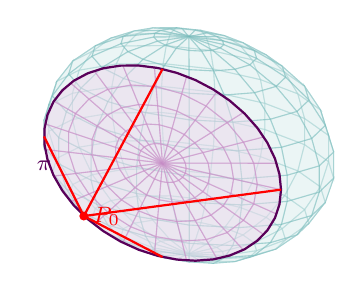
\begin{tikzpicture}
\begin{axis}[hide axis, view={120}{25}, width=7cm, height=7cm]
% 구면
\addplot3[
    surf, shader=faceted, faceted color=teal!55, fill=teal!12, opacity=0.4,
    domain=0:180, domain y=0:360, samples=14, samples y=18, z buffer=sort,
]
({1.5*sin(x)*cos(y)}, {1.5*sin(x)*sin(y)}, {1.5*cos(x)});
% 극면(원판, x=0.75 평면)
\addplot3[
    surf, shader=faceted, faceted color=violet!45, fill=violet!15, opacity=0.5,
    domain=0:1, domain y=0:360, samples=6, samples y=24, z buffer=sort,
]
({0.75}, {1.299*x*cos(y)}, {1.299*x*sin(y)});
% 접원(접점들의 자취) 경계선 강조
\addplot3[thick, violet!70!black, domain=0:360, samples=40, samples y=0]
({0.75}, {1.299*cos(x)}, {1.299*sin(x)});
% 극 P0
\addplot3[only marks, mark=*, mark size=1.4pt, red] coordinates {(3,0,0)};
% 접선(접원 위 네 점을 향해)
\addplot3[thick, red] coordinates {(3,0,0) (0.75,1.299,0)};
\addplot3[thick, red] coordinates {(3,0,0) (0.75,-1.299,0)};
\addplot3[thick, red] coordinates {(3,0,0) (0.75,0,1.299)};
\addplot3[thick, red] coordinates {(3,0,0) (0.75,0,-1.299)};
\node at (axis cs:3,0,0)[anchor=west, red]{\footnotesize $P_0$};
\node at (axis cs:0.75,-1.299,-0.4)[violet!70!black]{\footnotesize $\pi$};
\end{axis}
\end{tikzpicture}
\caption{구면 밖의 점 $P_0$(극)에서 그은 접선들이 구면과 닿는 접점들은 모두 하나의 원 위에 있고, 그 원이 놓인 평면 $\pi$가 $P_0$의 극면이다}
\end{figure}

\begin{tcolorbox}[
    colback=red!4,
    colframe=red!60!black,
    title=정리 1,
    fonttitle=\bfseries,
    boxrule=0.5mm,
    arc=3mm
    ]
    한 이차곡면에 관하여 점 \(P_1\)의 극면 \(\pi_1\)이 점 \(P_2\)를 지나면, 점 \(P_2\)의 극면 \(\pi_2\)는 점 \(P_1\)을 지난다.
\end{tcolorbox}

\begin{proof}
점 \(P_1(x_1,y_1,z_1)\)의 극면 \(\pi_1\)은
\[
ax_1x+by_1y+cz_1z+f(y_1z+yz_1)+g(z_1x+zx_1)+h(x_1y+xy_1)+l(x+x_1)+m(y+y_1)+n(z+z_1)+d=0
\]
이고, 이 평면이 \(P_2(x_2,y_2,z_2)\)를 지나면
\[
ax_1x_2+by_1y_2+cz_1z_2+f(y_1z_2+y_2z_1)+g(z_1x_2+z_2x_1)+h(x_1y_2+x_2y_1)+l(x_2+x_1)+m(y_2+y_1)+n(z_2+z_1)+d=0
\]
이 성립한다. 이 식은 \(1\leftrightarrow2\) 첨자 교환에 대해 대칭이므로, 이는 곧 \(P_2\)의 극면 \(\pi_2\)가 \(P_1\)을 지남을 뜻한다.
\end{proof}

\subsection*{EXAMPLE 1}
한 유심이차곡면에 관한 점 \(P_0\)의 극면 \(\pi\)는, 점 \(P_0\)와 중심을 잇는 직선을 종선으로 하는 경면에 평행함을 증명하여라.\\
\textbf{SOLUTION:} 타원면 \(\dfrac{x^2}{a^2}+\dfrac{y^2}{b^2}+\dfrac{z^2}{c^2}=1\)에 대하여 증명하자. 점 \(P_0(x_0,y_0,z_0)\)의 극면은
\[
\frac{x_0x}{a^2}+\frac{y_0y}{b^2}+\frac{z_0z}{c^2}=1
\]
한편, \(P_0\)와 원점을 잇는 직선을 종선으로 하는 경면의 방정식은
\[
\frac{x_0x}{a^2}+\frac{y_0y}{b^2}+\frac{z_0z}{c^2}=0
\]
이므로(상수항만 다름) 두 평면은 평행하다.

\subsection*{EXAMPLE 2 (멱, power of a point)}
정점 \(A(\alpha,\beta,\gamma)\)를 지나는 직선 \(g\)가 구면 \(F(x,y,z)=x^2+y^2+z^2+2ax+2by+2cz+d=0\)과 만나는 점을 \(P,Q\)라 할 때, \(\overline{AP}\cdot\overline{AQ}\)를 \(A\)의 \textbf{멱}(power)이라 한다. 이 멱이 상수임을 증명하여라.\\
\textbf{SOLUTION:} 직선 \(g\)의 방향코사인을 \(\lambda,\mu,\nu\)라 하면 \(x=\alpha+\lambda t,y=\beta+\mu t,z=\gamma+\nu t\)를 구면의 방정식에 대입하고 \(\lambda^2+\mu^2+\nu^2=1\)을 쓰면
\[
t^2+2(\alpha\lambda+\beta\mu+\gamma\nu+a\lambda+b\mu+c\nu)t+F(\alpha,\beta,\gamma)=0
\]
이므로 교점 \(P,Q\)에 대응하는 \(t\)값 \(\overline{AP},\overline{AQ}\)는 이 이차방정식의 두 근이다. 근과 계수의 관계에서
\[
\overline{AP}\cdot\overline{AQ}=F(\alpha,\beta,\gamma)\ (\text{일정})
\]

\subsection*{EXAMPLE 3 (근평면, radical plane)}
두 구면 \(F_1=x^2+y^2+z^2+2a_1x+2b_1y+2c_1z+d_1=0\), \(F_2=x^2+y^2+z^2+2a_2x+2b_2y+2c_2z+d_2=0\)에 대하여, 이들에 관한 멱이 같은 점의 자취를 구하여라.\\
\textbf{SOLUTION:} 자취 위의 점 \(P(x,y,z)\)는 \(F_1(x,y,z)=F_2(x,y,z)\)를 만족해야 하므로
\[
2(a_1-a_2)x+2(b_1-b_2)y+2(c_1-c_2)z+(d_1-d_2)=0
\]
이는 평면이며, 이를 \textbf{근평면}(radical plane)이라 한다.

\section*{[2] 선직면 (Ruled Surface)}

\begin{tcolorbox}[
    colback=teal!4,
    colframe=teal!65!black,
    title=정의 \& 핵심 규칙,
    fonttitle=\bfseries,
    boxrule=0.5mm,
    arc=3mm
    ]
    \textbf{\textcolor{teal!65!black}{정의.}}\quad
    곡면 자체가 그 위에 놓인 직선들(\textbf{모선}, generating line)로 가득 채워질 때, 이 곡면을 \textbf{선직면}(ruled surface)이라 한다.

    \noindent\textcolor{teal!50!black}{\rule{\linewidth}{0.4pt}}

    \textbf{\textcolor{teal!65!black}{핵심 규칙.}}\quad
    이차곡면 중 \textbf{자기 자신 위에 직선을 포함할 수 있는 것은 일엽쌍곡면, 쌍곡포물면, 추면, 주면 뿐}이다. (타원면·이엽쌍곡면·타원포물면은 불가능.)
\end{tcolorbox}

\textbf{판별.} 직선 \(x=x_0+\lambda t,y=y_0+\mu t,z=z_0+\nu t\)가 곡면 전체에 포함되려면, 대입해서 얻는 이차방정식이 \(t\)에 대해 \textbf{항등적으로 0}이어야 하므로 세 조건
\[
a\lambda^2+b\mu^2+c\nu^2+2f\mu\nu+2g\nu\lambda+2h\lambda\mu=0,\quad
(ax_0+hy_0+gz_0+l)\lambda+\cdots=0,\quad F(x_0,y_0,z_0)=0
\]
을 동시에 만족해야 한다.

\textbf{(i) 타원면·쌍곡면 \(ax^2+by^2+cz^2=1\ (abc\ne0)\):} 위 조건을 정리하면 \(abc<0\)이어야 하는데, \(a,b,c\)가 모두 음수일 수는 없으므로 둘은 양수, 하나는 음수여야 한다. 즉 부호가 \((+,+,-)\) 형태 -- 이는 \textbf{일엽쌍곡면뿐}이다.

\textbf{(ii) 포물면 \(ax^2+by^2+2nz=0\):} 조건 \(a\lambda^2+b\mu^2=0\)에서 \(a,b\)는 서로 다른 부호여야 한다. 즉 \textbf{쌍곡포물면뿐}이다.

\textbf{(iii) 추면·주면:} 도선을 지나는 모선 자체가 이미 직선이므로 자명하게 선직면이다.

% ============ 이미지 삽입 위치: 판별 결론 직후 -- 일엽쌍곡면이 직선들로 이루어짐을 시각화 ============
% 일엽쌍곡면 표면(청록, 반투명) 위에 실제로 놓이는 직선족(주황) 8개를 겹쳐 그림.
% "곡면이 휘어 보이지만 사실 직선들로 채워져 있다"는 선직면의 핵심을 시각적으로 보여줌.
\begin{figure}[h]
\centering
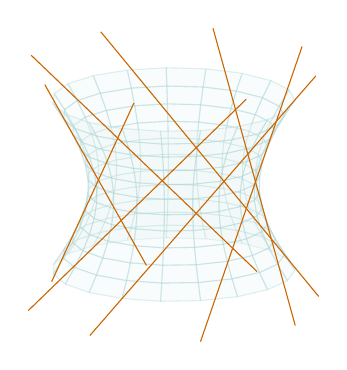
\begin{tikzpicture}
\begin{axis}[hide axis, view={115}{15}, width=6.5cm, height=6.5cm]
\addplot3[
    surf, shader=faceted, faceted color=teal!35, fill=teal!8, opacity=0.35,
    domain=-1:1, domain y=0:360, samples=12, samples y=20, z buffer=sort,
]
({1.3*sqrt(1+x^2)*cos(y)}, {1.3*sqrt(1+x^2)*sin(y)}, {2*x});
\addplot3[thin, orange!80!black] coordinates {(1.3,-1.82,-2.8) (1.3,1.82,2.8)};
\addplot3[thin, orange!80!black] coordinates {(2.206,-0.368,-2.8) (-0.368,2.206,2.8)};
\addplot3[thin, orange!80!black] coordinates {(1.82,1.3,-2.8) (-1.82,1.3,2.8)};
\addplot3[thin, orange!80!black] coordinates {(0.368,2.206,-2.8) (-2.206,-0.368,2.8)};
\addplot3[thin, orange!80!black] coordinates {(-1.3,1.82,-2.8) (-1.3,-1.82,2.8)};
\addplot3[thin, orange!80!black] coordinates {(-2.206,0.368,-2.8) (0.368,-2.206,2.8)};
\addplot3[thin, orange!80!black] coordinates {(-1.82,-1.3,-2.8) (1.82,-1.3,2.8)};
\addplot3[thin, orange!80!black] coordinates {(-0.368,-2.206,-2.8) (2.206,0.368,2.8)};
\end{axis}
\end{tikzpicture}
\caption{일엽쌍곡면(청록 곡면)이 실제로는 직선(모선, 주황)들의 집합으로 이루어져 있음을 보여주는 그림}
\end{figure}

\begin{figure}[h]
\centering
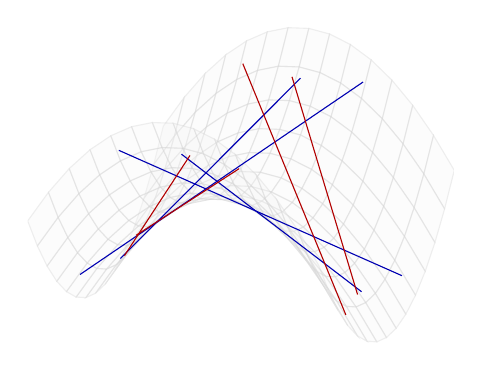
\begin{tikzpicture}
\begin{axis}[hide axis, view={115}{20}, width=7cm, height=7cm]
\addplot3[
    surf, shader=faceted, faceted color=gray!35, fill=gray!8, opacity=0.35,
    domain=-1.4:1.4, domain y=-1.4:1.4, samples=15, samples y=15,
]
{x^2-y^2};
\addplot3[thin, blue!70!black] coordinates {(-0.579, 1.279, -1.3) (1.279, -0.579, 1.3)};
\addplot3[thin, blue!70!black] coordinates {(-0.041, 1.141, -1.3) (1.141, -0.041, 1.3)};
\addplot3[thin, blue!70!black] coordinates {(0.579, -1.279, -1.3) (-1.279, 0.579, 1.3)};
\addplot3[thin, blue!70!black] coordinates {(0.041, -1.141, -1.3) (-1.141, 0.041, 1.3)};
\addplot3[thin, red!70!black] coordinates {(-0.579, -1.279, -1.3) (1.279, 0.579, 1.3)};
\addplot3[thin, red!70!black] coordinates {(-0.041, -1.141, -1.3) (1.141, 0.041, 1.3)};
\addplot3[thin, red!70!black] coordinates {(0.579, 1.279, -1.3) (-1.279, -0.579, 1.3)};
\addplot3[thin, red!70!black] coordinates {(0.041, 1.141, -1.3) (-1.141, -0.041, 1.3)};
\end{axis}
\end{tikzpicture}
\caption{쌍곡포물면(안장면)은 두 방향의 직선군(파랑·빨강)이 교차하며 곡면 전체를 이룬다}
\end{figure}

\textbf{모선의 명시적 형태.} 일엽쌍곡면 \(\dfrac{x^2}{a^2}+\dfrac{y^2}{b^2}-\dfrac{z^2}{c^2}=1\)은
\[
\left(\frac{x}{a}+\frac{z}{c}\right)\left(\frac{x}{a}-\frac{z}{c}\right)=\left(1+\frac{y}{b}\right)\left(1-\frac{y}{b}\right)
\]
로 쓸 수 있으므로, \(k\ne0\)인 상수마다
\[
\frac{x}{a}+\frac{z}{c}=k\left(1+\frac{y}{b}\right),\qquad \frac{x}{a}-\frac{z}{c}=\frac{1}{k}\left(1-\frac{y}{b}\right)
\]
로 정해지는 직선과,
\[
\frac{x}{a}+\frac{z}{c}=k\left(1-\frac{y}{b}\right),\qquad \frac{x}{a}-\frac{z}{c}=\frac{1}{k}\left(1+\frac{y}{b}\right)
\]
로 정해지는 직선이 모두 곡면 위에 놓인다. 즉 일엽쌍곡면은 \textbf{두 종류의 직선군}을 포함한다.

쌍곡포물면 \(\dfrac{x^2}{a^2}-\dfrac{y^2}{b^2}=2cz\)도 마찬가지로
\[
\left(\frac{x}{a}+\frac{y}{b}\right)\left(\frac{x}{a}-\frac{y}{b}\right)=2cz
\]
에서 \(k\ne0\)인 상수마다
\[
\frac{x}{a}+\frac{y}{b}=2ck\,z,\quad \frac{x}{a}-\frac{y}{b}=\frac{1}{k}
\qquad\text{및}\qquad
\frac{x}{a}+\frac{y}{b}=k,\quad \frac{x}{a}-\frac{y}{b}=\frac{2z}{ck}
\]
로 정해지는 두 종류의 직선군을 포함한다.

\section*{연습문제 7.6}
\begin{enumerate}
    \item 한 이차곡면에 관하여 일직선 위의 점들에 대한 극면들은 모두 다른 일직선을 포함함을 증명하여라.
    \item 한 이차곡면에 관하여 일직선을 포함하는 평면의 극은 모두 다른 일직선 위에 있음을 증명하여라.
    \item 두 구면의 중심을 잇는 직선은 두 구면의 근평면에 수직임을 증명하여라.
    \item 쌍곡포물면 \(x^2-y^2+z=0\)의 두 종류의 모선을 구하여라.
\end{enumerate}
\end{document}